% !TeX root = ../main.tex
\titlespacing{\chapter}{0cm}{-2cm}{0cm}
\chapter{實驗結果}


\section{實際晶片量測}
演算法於電腦上通過RS-232\cite{RS232}控制光源,對光譜晶片模組進行波長校正,ROI Scan後結果如圖\ref{fig:ROI SCAN 1}. 所示,精準的找到光源的ROI區域。

\begin{figure}[H]
	\vspace{0.8cm}
	\centering
	\begin{subfigure}[fig nice]{0.328\textwidth}
		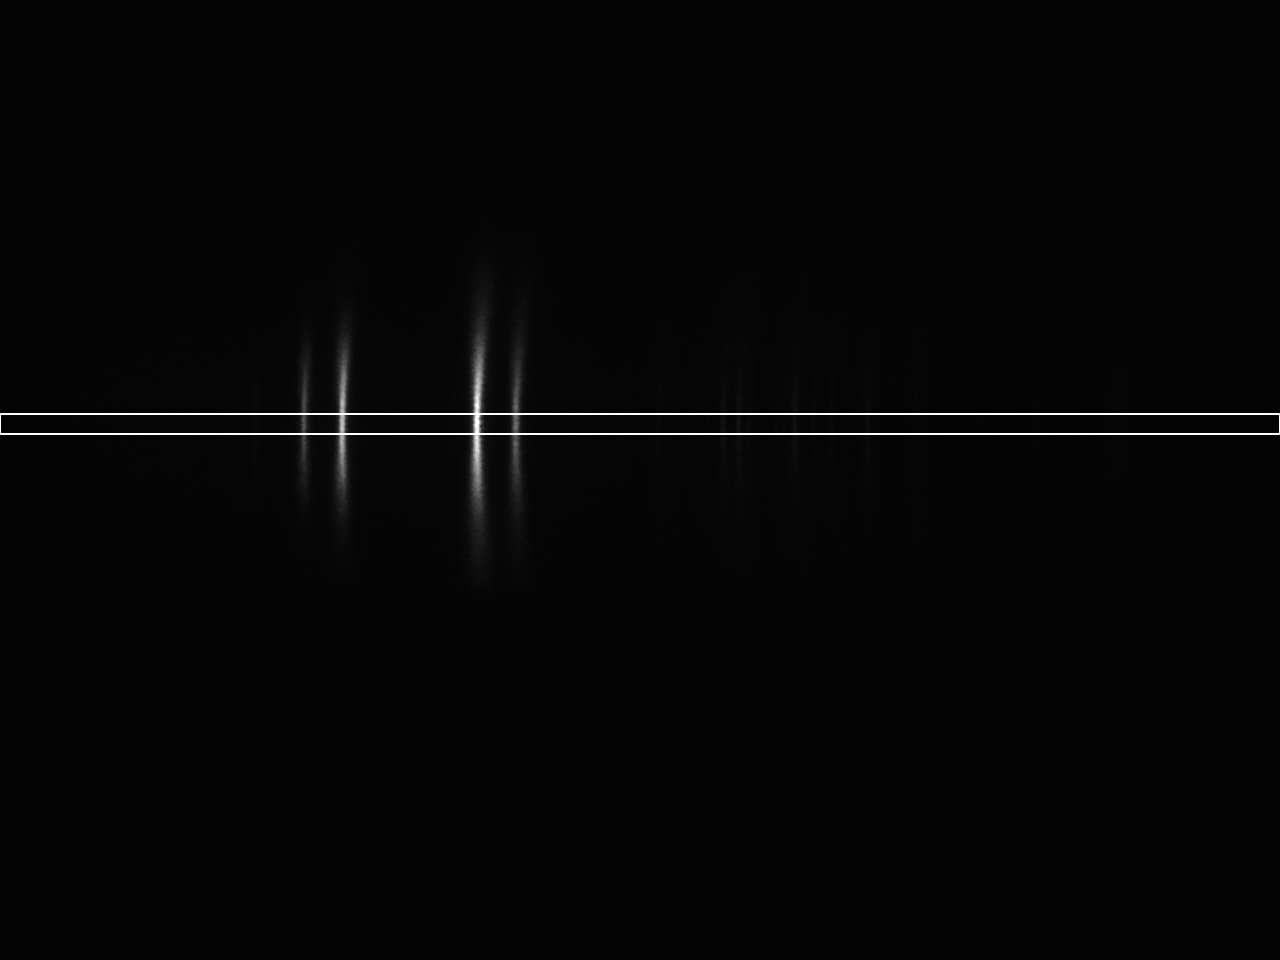
\includegraphics[width=4.9cm]{figures/Result/20C4-205-C4_full_Image__Hg_Ar_2021-05-10-16-25.jpg}
		\caption{}
		%\caption{汞氬燈}
		\label{fig:image_HG1}
	\end{subfigure}
	\begin{subfigure}[fig nice]{0.328\textwidth}
		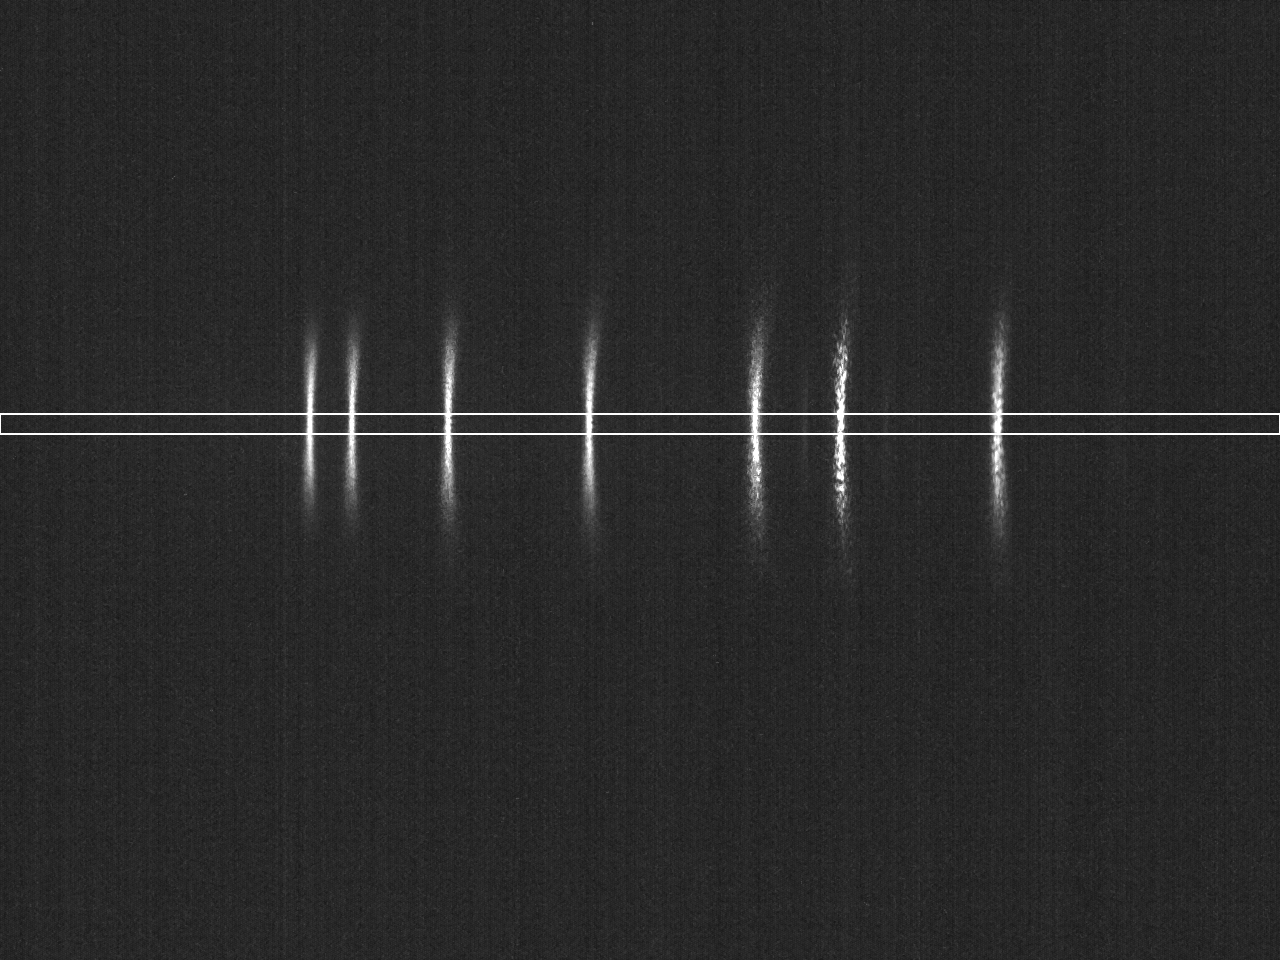
\includegraphics[width=4.9cm]{figures/Result/20C4-205-C4_full_Image__Laser8_2021-05-10-16-28.jpg}
		\caption{}
		%\caption{雷射}
		\label{fig:image_LASER1}
	\end{subfigure}
	\begin{subfigure}[fig nice]{0.328\textwidth}
		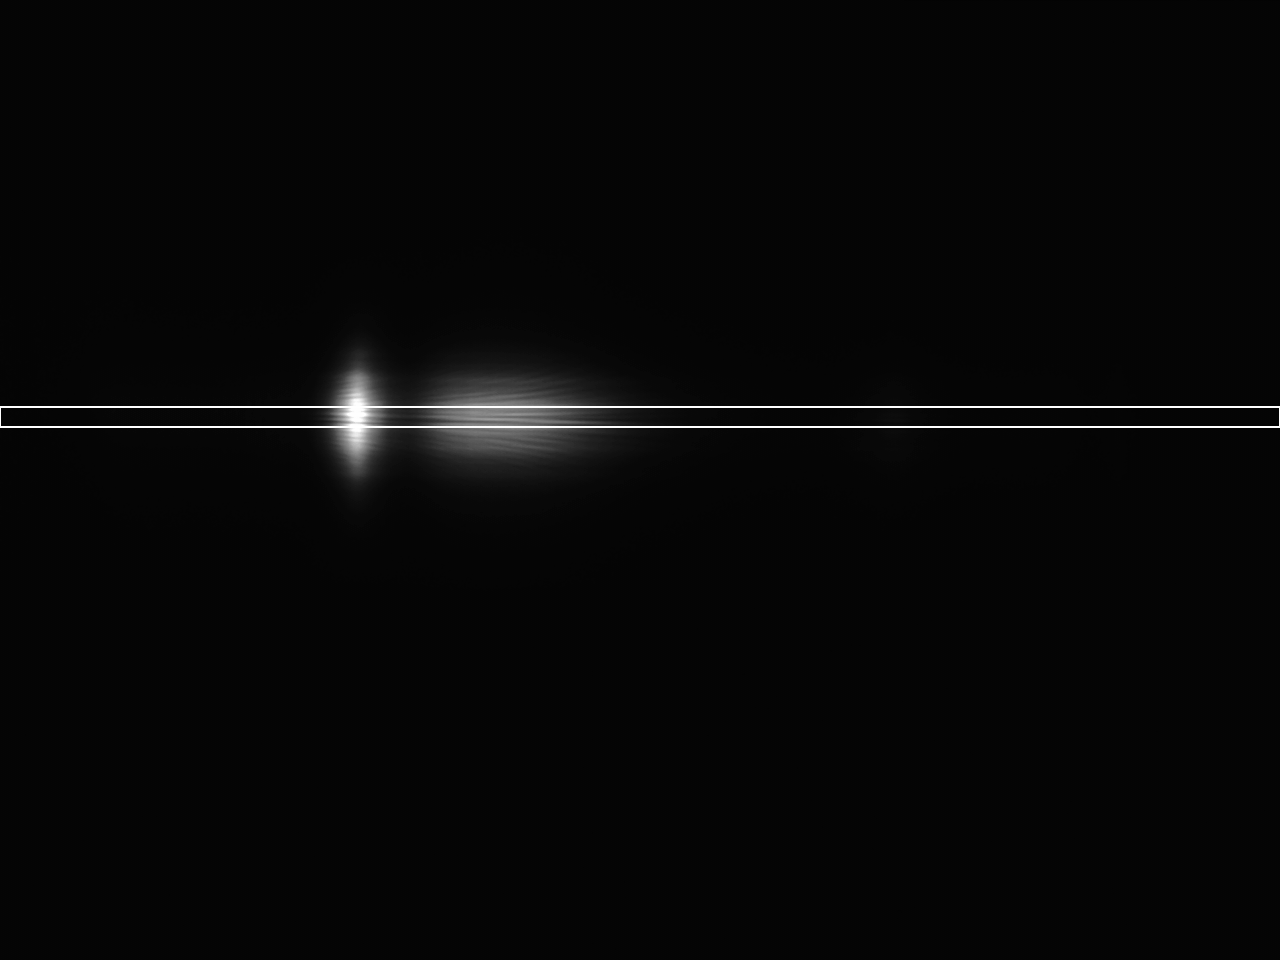
\includegraphics[width=4.9cm]{figures/Result/20C4-205-C4_full_Image__White_2021-05-10-16-30.jpg}
		\caption{}
		%\caption{白光LED}
		\label{fig:image_White1}
	\end{subfigure}
	\caption[同一晶片下不同光源的ROI SCAN結果圖]{同晶片不同光源ROI SCAN結果 (a)汞氬燈(b)雷射(c)白光LED}
	\label{fig:ROI SCAN 1}
\end{figure} 
在同一晶片下,通過將ROI區域影像中所有像素點帶入式(\ref{eq:2.4})計算得出如式(\ref{RGB:3.9})之光譜數據矩陣後,繪出光譜圖。汞氬燈、雷射與白光各自的光譜波形圖如圖\ref{fig:Spectrum 1}. 所示。
\begin{figure}[H]
	\vspace{0.8cm}
	\centering
	\begin{subfigure}[fig nice]{0.328\textwidth}
		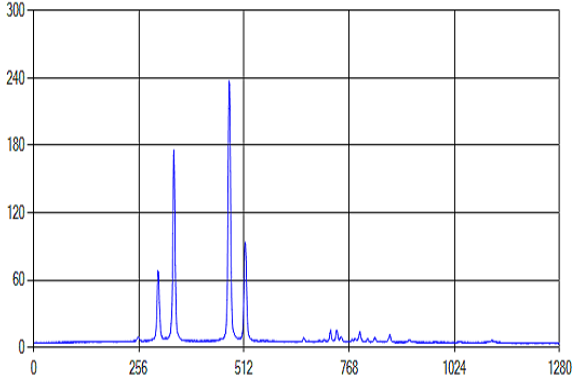
\includegraphics[width=4.9cm]{figures/Result/20C4-205-C4_HgAr.PNG}
		\caption{}
		%\caption{汞氬燈}
		\label{fig:Spectrum_HG1}
	\end{subfigure}
	\begin{subfigure}[fig nice]{0.328\textwidth}
		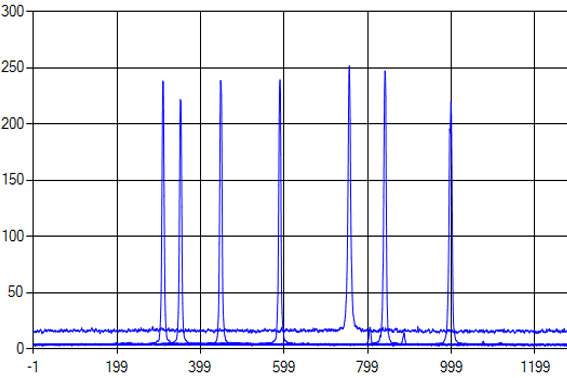
\includegraphics[width=4.9cm]{figures/Result/20C4-205-C4_Laser.PNG}
		\caption{}
		%\caption{七根單雷射疊圖}
		\label{fig:Spectrum_LASER1}
	\end{subfigure}
	\begin{subfigure}[fig nice]{0.328\textwidth}
		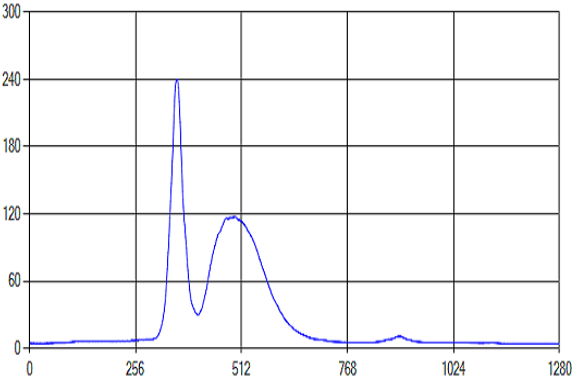
\includegraphics[width=4.9cm]{figures/Result/20C4-205-C4_White.PNG}
		\caption{}
		%\caption{白光LED}
		\label{fig:Spectrum_White1}
	\end{subfigure}
	\caption[同一晶片下不同光源的光譜圖形]{同晶片不同光源的光譜圖形 (a)汞氬燈(b)七根單雷射疊圖(c)白光LED}
	\label{fig:Spectrum 1}
\end{figure} 
\newpage
經演算法計算後汞氬燈與雷射峰值偵測與波長校正三次多項式擬合的結果如圖\ref{峰值偵測與三次多項式擬合結果}. 所示。汞氬燈光譜波形量化結果,如圖\ref{汞燈光譜量化}. 所示。白光光譜波形量化結果,如圖\ref{白光光譜量化}. 所示。晶片參數如表\ref{不同晶片汞氬燈校正結果參數}. 所示。
\begin{figure}[H] %H为当前位置,!htb为忽略美学标准,htbp为浮动图形
	\centering %图片居中
	\vspace{0.8cm}
	%\setlength{\abovecaptionskip}{1cm}
	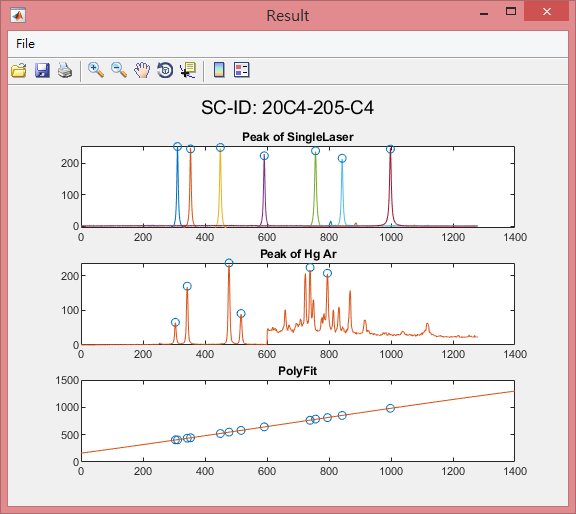
\includegraphics[width=0.74\textwidth]{figures/Result/Result_2021-05-10-16-29-08.jpg} %插入图片,[]中设置图片大小,{}中是图片文件名
	\caption{峰值偵測與三次多項式擬合結果} %最终文档中希望显示的图片标题
	\label{峰值偵測與三次多項式擬合結果} %用于文内引用的标签
\end{figure}
\begin{figure}[H] %H为当前位置,!htb为忽略美学标准,htbp为浮动图形
	\centering %图片居中
	\vspace{0.8cm}
	%\setlength{\abovecaptionskip}{1cm}
	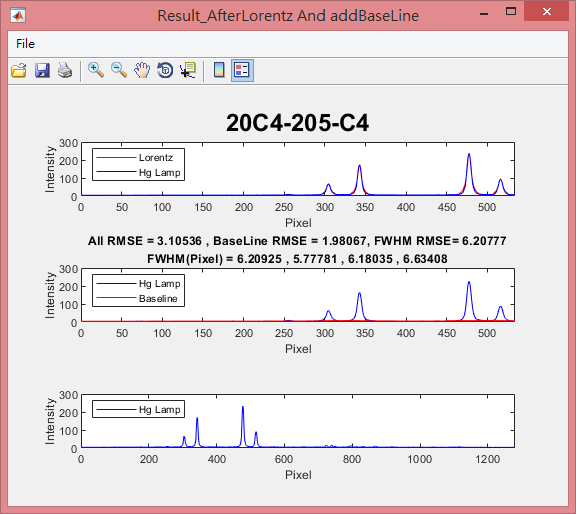
\includegraphics[width=0.74\textwidth]{figures/Result/Result_2021-05-10-16-24-49.jpg} %插入图片,[]中设置图片大小,{}中是图片文件名
	\caption{汞燈光譜量化} %最终文档中希望显示的图片标题
	\label{汞燈光譜量化} %用于文内引用的标签
\end{figure}
\begin{figure}[H] %H为当前位置,!htb为忽略美学标准,htbp为浮动图形
	\centering %图片居中
	\vspace{0.8cm}
	%\setlength{\abovecaptionskip}{1cm}
	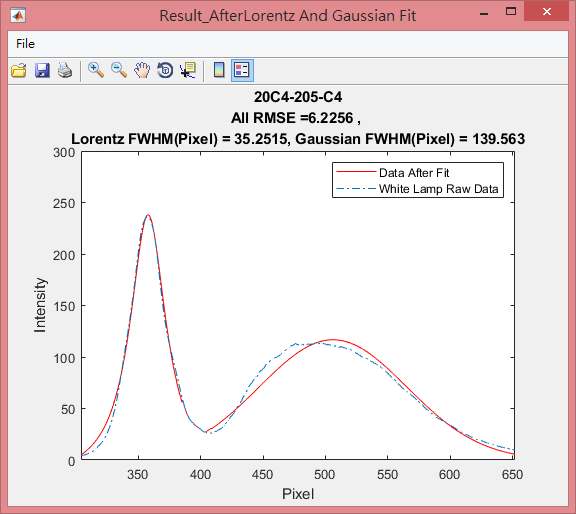
\includegraphics[width=0.74\textwidth]{figures/Result/Result_2021-05-10-16-30-57.jpg} %插入图片,[]中设置图片大小,{}中是图片文件名
	\caption{白光光譜量化} %最终文档中希望显示的图片标题
	\label{白光光譜量化} %用于文内引用的标签
\end{figure}
\begin{center}
	\vspace{0.8cm}
	\captionof{table}{晶片20C4-205-C4校正結果參數表}\label{不同晶片汞氬燈校正結果參數}
\begin{tabularx}{\textwidth}{cccccccc}
	\hline\hline
	\multicolumn{8}{c}{空間轉換方程式}\\
	\hline
	\multicolumn{8}{c}{$\lambda_i = 161.702366565752 + 0.76016P_i + 12.26498\times 10^{-5}P_i^2 -6.16582\times 10^{-8}P_i^3$}\\
	\hline
	\multirow{2}{*}{光源}
	&峰值位置&標準波長&轉換波長&誤差&半高全寬&半高全寬&解析度\\
	&(pixel)&(nm)&(nm)&(nm)&(pixel)&(nm)&(nm)\\
	\hline
	\multirow{4}{*}{汞燈 }
	&304.42&404.65&404.59&-0.06&5.81&4.76&5.18\\
	&342.70&435.83&435.91&0.08&6.32&5.17&5.18\\
	&477.45&546.07&546.10&0.03&6.49&5.32&5.18\\
	&516.24&578.01&577.93&-0.08&6.61&5.43&5.18\\
	\hline
	\multirow{2}{*}{氬燈 }
	&738.97&763.51&763.57&0.06&6.49&5.51&5.18\\
	&795.04&811.53&811.49&0.04&7.30&6.28&5.18\\  
	\hline	
	雷射1&311.41&404.97&406.21&1.24&5.09&4.26&4.18\\
	雷射2&353.37&443.93&441.41&-2.52&5.13&4.31&4.18\\
	雷射3&449.50&520.69&522.45&1.76&5.49&4.64&4.18\\
	雷射5&591.20&642.13&642.35&0.22&5.45&4.61&4.18\\
	雷射6&756.55&784.46&781.74&-2.72&6.39&5.35&4.18\\
	雷射7&842.54&851.04&853.50&2.46&5.43&4.51&4.18\\
	雷射8&998.17&981.67&981.25&-0.42&6.44&5.21&4.18\\
	\hline\hline
\end{tabularx}
\end{center}
\newpage
\section{不同方法之波長校正比較}
將多個不同晶片的量測進行進一步比較,波長校正參數由汞氬燈與雷射此兩光源所提供的波峰進行擬合,比較單純以汞氬燈或雷射波峰進行波長校正的準確度,與使用雙光源所提供的波峰進行的波長校正的準確度的差異。\par
汞氬燈波峰偵測與三次多項式擬合結果如圖\ref{C4汞氬燈峰值偵測與擬合曲線}. 至圖\ref{B4晶片汞氬燈峰值偵測與擬合曲線}. 所示,波峰詳細參數如表\ref{不同晶片校正波峰參數表}. 所示。

\begin{figure}[H] %H为当前位置,!htb为忽略美学标准,htbp为浮动图形
	\centering %图片居中
	\vspace{0.8cm}
	%\setlength{\abovecaptionskip}{1cm}
	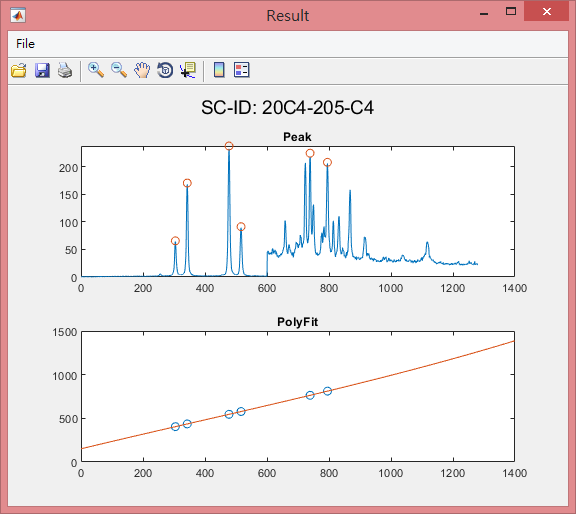
\includegraphics[width=0.74\textwidth]{figures/Result/比較/C4.jpg} %插入图片,[]中设置图片大小,{}中是图片文件名
	\caption{20C4-205-C4晶片汞氬燈峰值偵測與擬合曲線} %最终文档中希望显示的图片标题
	\label{C4汞氬燈峰值偵測與擬合曲線} %用于文内引用的标签
\end{figure}
\begin{figure}[H] %H为当前位置,!htb为忽略美学标准,htbp为浮动图形
	\centering %图片居中
	\vspace{0.8cm}
	%\setlength{\abovecaptionskip}{1cm}
	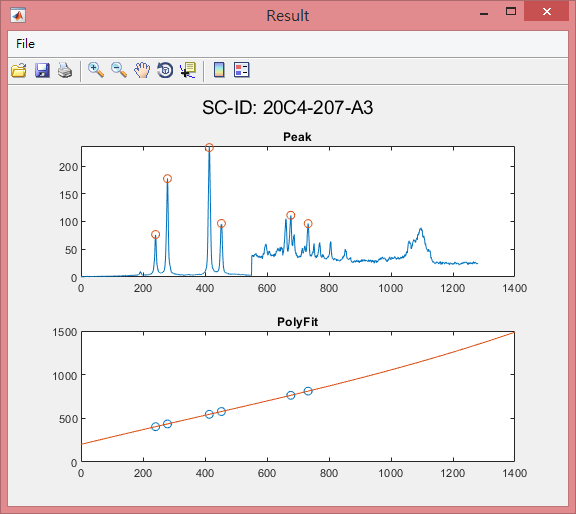
\includegraphics[width=0.74\textwidth]{figures/Result/比較/A3.jpg} %插入图片,[]中设置图片大小,{}中是图片文件名
	\caption{20C4-207-A3晶片汞氬燈峰值偵測與擬合曲線} %最终文档中希望显示的图片标题
	\label{A3汞氬燈峰值偵測與擬合曲線} %用于文内引用的标签
\end{figure}
\begin{figure}[H] %H为当前位置,!htb为忽略美学标准,htbp为浮动图形
	\centering %图片居中
	\vspace{0.8cm}
	%\setlength{\abovecaptionskip}{1cm}
	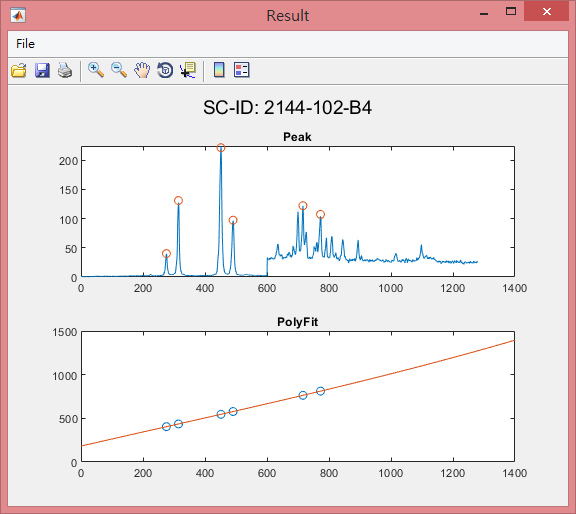
\includegraphics[width=0.74\textwidth]{figures/Result/比較/B4.jpg} %插入图片,[]中设置图片大小,{}中是图片文件名
	\caption{2144-102-B4晶片汞氬燈峰值偵測與擬合曲線} %最终文档中希望显示的图片标题
	\label{B4晶片汞氬燈峰值偵測與擬合曲線} %用于文内引用的标签
\end{figure}

\begin{center}
	\vspace{0.8cm}
	\captionof{table}{不同晶片校正波峰參數表}\label{不同晶片校正波峰參數表}
\begin{tabularx}{\textwidth}{m{0.14\textwidth}<{\centering}m{0.19\textwidth}<{\centering}m{0.19\textwidth}<{\centering}m{0.19\textwidth}<{\centering}m{0.15\textwidth}<{\centering}}
	\hline\hline
	晶片ID&20C4-205-C4&20C4-207-A3&2144-102-B4&\\
	\hline
	\multirow{2}{*}{光源}
	&峰值位置&峰值位置&峰值位置&標準波長\\
	&(pixel)&(pixel)&(pixel)&(nm)\\
	\hline
	\multirow{4}{*}{汞燈 }
	&304.42&240.62 &275.53 &404.65\\
	&342.70&278.97 &314.45 &435.83\\
	&477.45&413.94 &451.45 &546.07\\
	&516.24&452.89 &490.53 &578.01\\
	\hline
	\multirow{2}{*}{氬燈 }
	&738.97&676.73 &715.87 &763.51\\
	&795.04&732.63 &772.62 &811.53\\ 
	\hline\hline
\end{tabularx}
\vspace{10pt}
\end{center}
\par
由圖\ref{C4汞氬燈峰值偵測與擬合曲線}. 至圖\ref{B4晶片汞氬燈峰值偵測與擬合曲線}. 可以看出單純使用汞氬燈擬合時,於800像素後並無波峰參考點,導致擬和曲線開始產生偏移。
接著是僅使用雷射進行波長校正,三個不同晶片的波峰偵測與三次多項式擬合結果如下列圖\ref{C4晶片雷射峰值偵測與擬合曲線}. 至圖\ref{B4晶片雷射峰值偵測與擬合曲線}. 所示,波峰參數如表\ref{不同晶片雷射校正波峰參數表}. 所示。
\begin{figure}[H] %H为当前位置,!htb为忽略美学标准,htbp为浮动图形
	\centering %图片居中
	\vspace{0.8cm}
	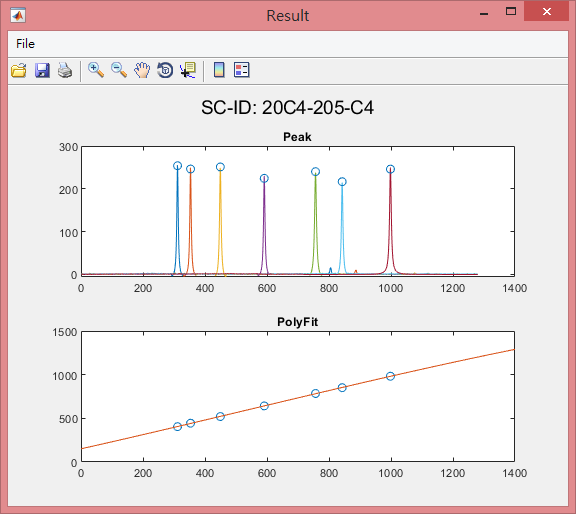
\includegraphics[width=0.7\textwidth]{figures/Result/比較/C4-L.jpg} %插入图片,[]中设置图片大小,{}中是图片文件名
	\caption{20C4-205-C4晶片雷射峰值偵測與擬合曲線} %最终文档中希望显示的图片标题
	\label{C4晶片雷射峰值偵測與擬合曲線} %用于文内引用的标签
\end{figure}
\begin{figure}[H] %H为当前位置,!htb为忽略美学标准,htbp为浮动图形
	\centering %图片居中
	\vspace{0.8cm}
	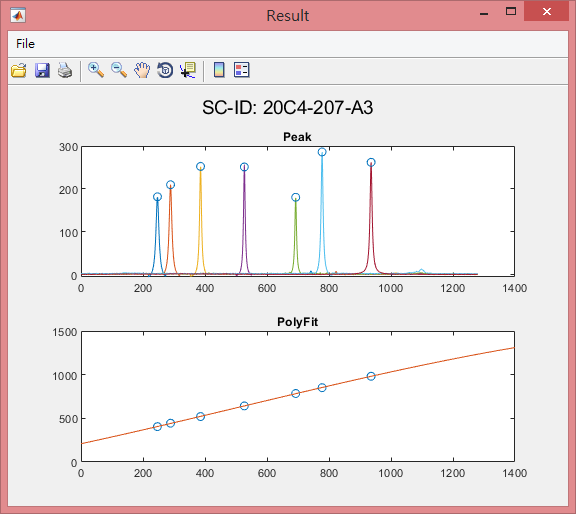
\includegraphics[width=0.7\textwidth]{figures/Result/比較/A3-L.jpg} %插入图片,[]中设置图片大小,{}中是图片文件名
	\caption{20C4-207-A3晶片雷射峰值偵測與擬合曲線} %最终文档中希望显示的图片标题
	\label{A3晶片雷射峰值偵測與擬合曲線} %用于文内引用的标签
\end{figure}
\begin{figure}[H] %H为当前位置,!htb为忽略美学标准,htbp为浮动图形
	\centering %图片居中
	\vspace{0.8cm}
	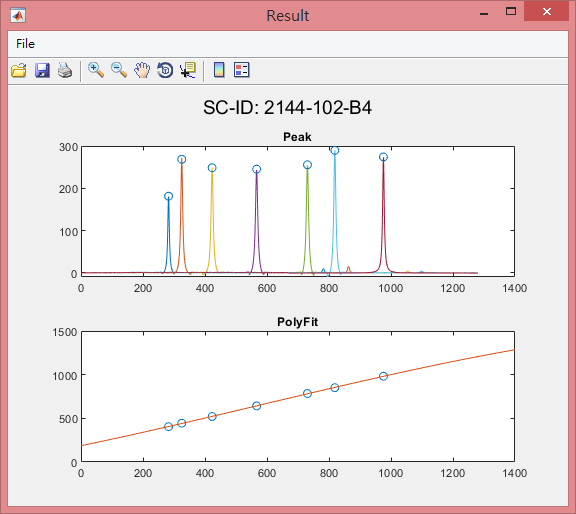
\includegraphics[width=0.7\textwidth]{figures/Result/比較/B4-L.jpg} %插入图片,[]中设置图片大小,{}中是图片文件名
	\caption{2144-102-B4晶片雷射峰值偵測與擬合曲線} %最终文档中希望显示的图片标题
	\label{B4晶片雷射峰值偵測與擬合曲線} %用于文内引用的标签
\end{figure}

\begin{center}
	\vspace{0.8cm}
	\captionof{table}{不同晶片雷射校正波峰參數表}\label{不同晶片雷射校正波峰參數表}
\begin{tabularx}{\textwidth}{m{0.14\textwidth}<{\centering}m{0.19\textwidth}<{\centering}m{0.19\textwidth}<{\centering}m{0.19\textwidth}<{\centering}m{0.15\textwidth}<{\centering}}
	\hline\hline
	晶片ID&20C4-205-C4&20C4-207-A3&2144-102-B4&\\
	\hline
	\multirow{2}{*}{光源}
	&峰值位置&峰值位置&峰值位置&標準波長\\
	&(pixel)&(pixel)&(pixel)&(nm)\\
	\hline
	雷射1&311.41&246.61&282.46&404.97\\
	雷射2&353.37&288.84&324.99&443.93\\
	雷射3&449.50&385.66&422.99&520.69\\
	雷射5&591.20&526.96&566.49&642.13\\
	雷射6&756.55&692.57&730.44&784.46\\
	雷射7&842.54&777.71&818.83&851.04\\
	雷射8&998.17&935.76&975.65&981.67\\
	\hline\hline
\end{tabularx}
\vspace{10pt}
\end{center}
\newpage
由圖\ref{C4晶片雷射峰值偵測與擬合曲線}. 至圖\ref{B4晶片雷射峰值偵測與擬合曲線}. 可以看出使用雷射擬合時,於800像素後仍有波峰參考點,因此擬合曲線在高波段時比起汞氬燈更為精確。
接著結合汞氬燈與各雷射所提供之波峰參考點進行擬合,結果如圖\ref{C4晶片結合校正擬合曲線}. 至圖\ref{B4晶片結合校正擬合曲線}. 所示。
\begin{figure}[H] %H为当前位置,!htb为忽略美学标准,htbp为浮动图形
	\centering %图片居中
	\vspace{0.8cm}
	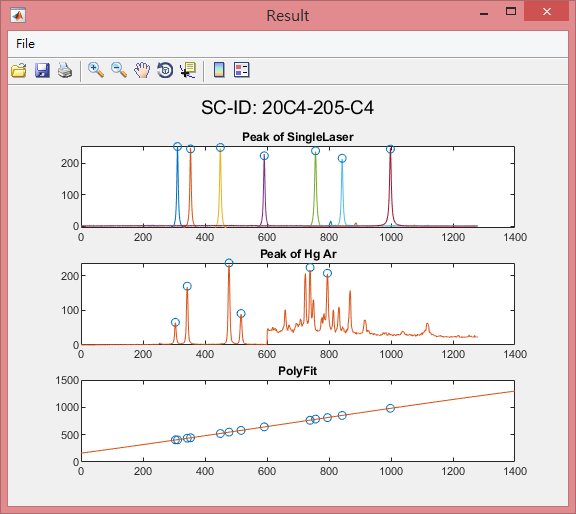
\includegraphics[width=0.7\textwidth]{figures/Result/比較/C4-COM.jpg} %插入图片,[]中设置图片大小,{}中是图片文件名
	\caption{20C4-205-C4晶片結合校正擬合曲線} %最终文档中希望显示的图片标题
	\label{C4晶片結合校正擬合曲線} %用于文内引用的标签
\end{figure}
\begin{figure}[H] %H为当前位置,!htb为忽略美学标准,htbp为浮动图形
	\centering %图片居中
	\vspace{0.8cm}
	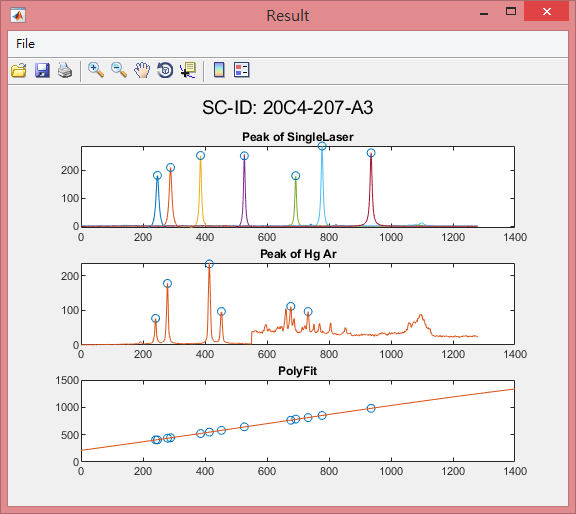
\includegraphics[width=0.7\textwidth]{figures/Result/比較/A3-COM.jpg} %插入图片,[]中设置图片大小,{}中是图片文件名
	\caption{20C4-207-A3晶片結合校正擬合曲線} %最终文档中希望显示的图片标题
	\label{A3晶片結合校正擬合曲線} %用于文内引用的标签
\end{figure}
\begin{figure}[H] %H为当前位置,!htb为忽略美学标准,htbp为浮动图形
	\centering %图片居中
	\vspace{0.8cm}
	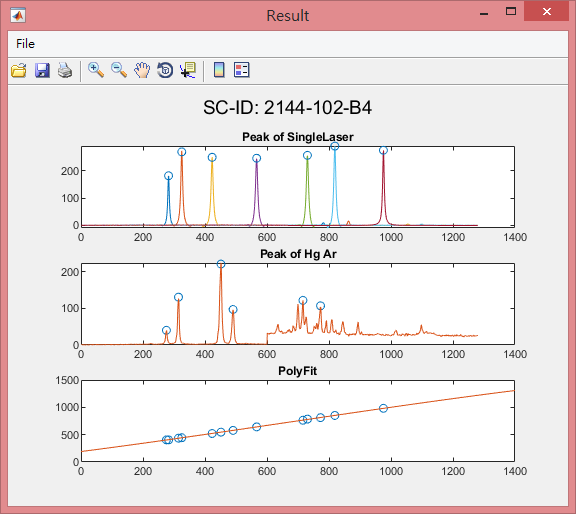
\includegraphics[width=0.7\textwidth]{figures/Result/比較/B4-COM.jpg} %插入图片,[]中设置图片大小,{}中是图片文件名
	\caption{2144-102-B4晶片結合校正擬合曲線} %最终文档中希望显示的图片标题
	\label{B4晶片結合校正擬合曲線} %用于文内引用的标签
\end{figure}
\newpage
晶片(20C4-205-C4)之汞氬燈、雷射與結合校正的轉換方程,如式(\ref{eq4.1})所示。將參考波峰像素位置pixel帶入式(\ref{eq4.1})轉換為波長nm,其偏差如表\ref{晶片20C4-205-C4三種校正方法比較表}. 所示。
\begin{equation}\label{eq4.1}
	\begin{cases}		
		& Hg Ar: \lambda(P) = 8.40\times 10^{-8}P^3 -9.63\times 10^{-5}P^2+0.854P+151.176\\
		& Laser: \lambda(P) = -5.84\times 10^{-8}P^3 + 9.47\times 10^{-5}P^2+0.795P+151.097\\
		& Combine: \lambda(P) = -6.17\times 10^{-8}P^3 + 12.26\times 10^{-5}P^2+0.76P+161.702\\
	\end{cases}
\end{equation}
\begin{center}
\captionof{table}{晶片20C4-205-C4三種校正方法比較表}\label{晶片20C4-205-C4三種校正方法比較表}
\begin{tabularx}{\textwidth}{cccccccc}
	\hline\hline
	晶片ID&\multicolumn{7}{c}{20C4-205-C4}\\%&\multicolumn{2}{c}{20C4-207-A3}&\multicolumn{2}{c}{2144-102-B4}\\
	\hline
	%校正方程&\multicolumn{7}{c}{----}\\
	%\hline
	校正方法&&\multicolumn{2}{c}{汞氬燈}&\multicolumn{2}{c}{雷射}&\multicolumn{2}{c}{結合校正}\\
	\hline
	    &標準波長&校正波長&偏差&校正波長&偏差&校正波長&偏差\\
	光源&(nm)   &(nm)    &(nm)&(nm)   &(nm)&(nm)   &(nm)\\
	\hline
	\multirow{6}{*}{汞氬燈}
	&404.65	&404.59	&0.06	&400.36	&4.29	&402.74	&1.91\\
	&435.83	&435.91	&-0.08	&432.44	&3.39	&434.14	&1.69\\
	&546.07	&546.10	&-0.03	&546.08	&-0.01	&545.89	&0.18\\
	&578.01	&577.93	&0.08	&578.90	&-0.89	&578.34	&-0.33\\
	&763.51	&763.57	&-0.06	&766.99	&-3.48	&765.54	&-2.03\\
	&811.53	&811.49	&0.04	&813.94	&-2.41	&812.61	&-1.08\\
	\hline
	\multirow{7}{*}{雷射}
	&404.97	&410.31	&-5.34	&406.21	&-1.24	&408.46	&-3.49\\
	&443.93	&444.63	&-0.70	&441.41	&2.52	&442.92	&1.01\\
	&520.69	&523.21	&-2.52	&522.45	&-1.76	&522.58	&-1.89\\
	&642.13	&639.76	&2.37	&642.35	&-0.22	&641.24	&0.89\\
	&784.46	&778.53	&5.9	&781.73	&2.73	&780.31	&4.15\\
	&851.04	&852.60	&-1.56	&853.50	&-2.46	&852.36	&-1.32\\
	&981.67	&991.23	&-9.56	&981.25	&0.42	&981.36	&0.31\\	
	\hline
	偏差RMS& & &3.61& &2.37& &1.93\\
	\hline\hline
\end{tabularx}
\end{center}


\newpage%......................................................................希望表格從下一頁開始排版
晶片(20C4-207-A3)之汞氬燈、雷射與結合校正的轉換方程,如式(\ref{eq4.2})所示。將參考波峰像素位置pixel帶入式(\ref{eq4.2})轉換為波長nm,其偏差如表\ref{晶片20C4-207-A3三種校正方法比較表}. 所示。
\begin{equation}\label{eq4.2}
	\begin{cases}		
		& Hg Ar: \lambda(P) = 1.30\times 10^{-7}P^3 -1.48\times 10^{-4}P^2+0.871P+201.698\\
		& Laser: \lambda(P) = -1.05\times 10^{-7}P^3 + 1.62\times 10^{-4}P^2+0.765P+209.287\\
		& Combine: \lambda(P) = -7.48\times 10^{-8}P^3 + 13.38\times 10^{-5}P^2+0.761P+213.265\\
	\end{cases}
\end{equation}
\begin{center}
	\vspace{0.5cm}
	\captionof{table}{晶片20C4-207-A3三種校正方法比較表}\label{晶片20C4-207-A3三種校正方法比較表}
\begin{tabularx}{\textwidth}{cccccccc}
	\hline\hline
	晶片ID&\multicolumn{7}{c}{20C4-207-A3}\\%\multicolumn{2}{c}{2144-102-B4}\\
	\hline
	%校正方程&\multicolumn{7}{c}{----}\\
	%\hline
	校正方法&&\multicolumn{2}{c}{汞氬燈}&\multicolumn{2}{c}{雷射}&\multicolumn{2}{c}{結合校正}\\
	\hline
	    &標準波長&校正波長&偏差&校正波長&偏差&校正波長&偏差\\
	光源&(nm)   &(nm)    &(nm)&(nm)   &(nm)&(nm)   &(nm)\\
	\hline
	\multirow{6}{*}{汞氬燈}
&404.65&404.53	&0.12	&401.34	&3.31	&403.17	&1.48\\
&435.83&436.00	&-0.17	&433.10	&2.73	&434.45	&1.38\\
&546.07&546.10	&-0.03	&546.38	&-0.31	&546.04	&0.03\\
&578.01&577.88	&0.13	&579.36	&-1.35	&578.57	&-0.56\\
&763.51&763.61	&-0.10	&768.87	&-5.36	&766.58	&-3.07\\
&811.53&811.47	&0.06	&815.67	&-4.14	&813.44	&-1.91\\
\hline
\multirow{7}{*}{雷射}
&404.97&409.46	&-4.49	&406.28	&-1.31	&408.04	&-3.07\\
&443.93&444.07	&-0.14	&441.31	&2.62	&442.53	&1.40\\
&520.69&523.06	&-2.37	&522.50	&-1.81	&522.50	&-1.81\\
&642.13&638.60	&3.53	&642.20	&-0.07	&640.67	&1.46\\
&784.46&777.09	&7.37	&782.17	&2.29	&779.87	&4.59\\
&851.04&850.68	&0.36	&853.11	&-2.07	&851.10	&-0.06\\
&981.67&993.61	&-11.94	&981.32	&0.35	&981.54	&0.13\\
	\hline
	偏差RMS& & &4.25& &2.59& &2.06\\
	\hline\hline
\end{tabularx}
\end{center}
\newpage
晶片(2144-102-B4)之汞氬燈、雷射與結合校正的轉換方程,如式(\ref{eq4.3})所示。將參考波峰像素位置pixel帶入式(\ref{eq4.3})轉換為波長nm,其偏差如表\ref{晶片2144-102-B4三種校正方法比較表}. 所示。
\begin{equation}\label{eq4.3}
	\begin{cases}		
		& Hg Ar: \lambda(P) = 5.65\times 10^{-8}P^3 -4.64\times 10^{-5}P^2+0.814P+182.491\\
		& Laser: \lambda(P) = -1.1\times 10^{-7}P^3 + 1.92\times 10^{-4}P^2+0.731P+186.997\\
		& Combine: \lambda(P) = -7.88\times 10^{-8}P^3 + 1.59\times 10^{-4}P^2+0.73P+191.36\\
	\end{cases}
\end{equation}
\begin{center}
	\vspace{0.5cm}
	\captionof{table}{晶片2144-102-B4三種校正方法比較表}\label{晶片2144-102-B4三種校正方法比較表}
\begin{tabularx}{\textwidth}{cccccccc}
	\hline\hline
	晶片ID&\multicolumn{7}{c}{2144-102-B4}\\
	\hline
	%校正方程&\multicolumn{7}{c}{----}\\
	%\hline
	校正方法&&\multicolumn{2}{c}{汞氬燈}&\multicolumn{2}{c}{雷射}&\multicolumn{2}{c}{結合校正}\\
	\hline
	    &標準波長&校正波長&偏差&校正波長&偏差&校正波長&偏差\\
	光源&(nm)   &(nm)    &(nm)&(nm)   &(nm)&(nm)   &(nm)\\
	\hline
	\multirow{6}{*}{汞氬燈}
&404.65&	404.62&	0.03	&400.76	&3.89	&402.90	&1.75\\
&435.83&	435.86&	-0.03	&432.51	&3.32	&434.15	&1.68\\
&546.07&	546.19&	-0.12	&546.15	&-0.08	&546.00	&0.07\\
&578.01&	577.86&	0.15	&578.94	&-0.93	&578.32	&-0.31\\
&763.51&	763.58&	-0.07	&768.57	&-5.06	&766.31	&-2.80\\
&811.53&	811.49&	0.04	&815.92	&-4.39	&813.69	&-2.16\\
\hline
\multirow{7}{*}{雷射}
&404.97&	410.18&	-5.21	&406.39	&-1.42	&408.44	&-3.47\\
&443.93&	444.32&	-0.39	&441.16	&2.77	&442.66	&1.27\\
&520.69&	523.20&	-2.51	&522.36	&-1.67	&522.56	&-1.87\\
&642.13&	639.79&	2.34	&642.90	&-0.77	&641.47	&0.66\\
&784.46&	775.83&	8.63	&780.76	&3.70	&778.48	&5.98\\
&851.04&	850.94&	0.10	&854.18	&-3.14	&852.17	&-1.13\\
&981.67&	988.20&	-6.53	&981.15	&0.52	&981.34	&0.33\\
	\hline
	偏差RMS& & &3.46& &2.89& &2.37\\
	\hline\hline
\end{tabularx}
\vspace{10pt}
\end{center}

由表\ref{晶片20C4-205-C4三種校正方法比較表}. 至表\ref{晶片2144-102-B4三種校正方法比較表}. 可以看出汞氬燈校正因波校正之參考波峰聚集於811nm前,因此在高波段區域偏差相當嚴重,而雷射校正因在981nm仍有參考波峰因此則無此問題,而結合校正同時納入所有汞氬燈與雷射所提供之參考波峰,故參考數據最多,因此所擬合出之轉換多項式將最為精準,轉換後之波長偏差也是三種方法中最低。
\par
為驗證所得之轉換方程式是否正確,現將所有像素即0至1280pixel,帶入此三個晶片各自的結合校正所得之空間轉換方程式,並各自取出其白光LED光譜數據,並將其各自轉換至波長空間後的白光LED光譜疊圖,並查看轉換至波長空間後的藍光波峰,是否正確落在藍光波峰的標準波長450nm,結果如圖\ref{三個晶片轉換至波長空間後的白光光譜疊圖}. 所示。
\begin{figure}[H] %H为当前位置,!htb为忽略美学标准,htbp为浮动图形
	\centering %图片居中
	\vspace{0.8cm}
	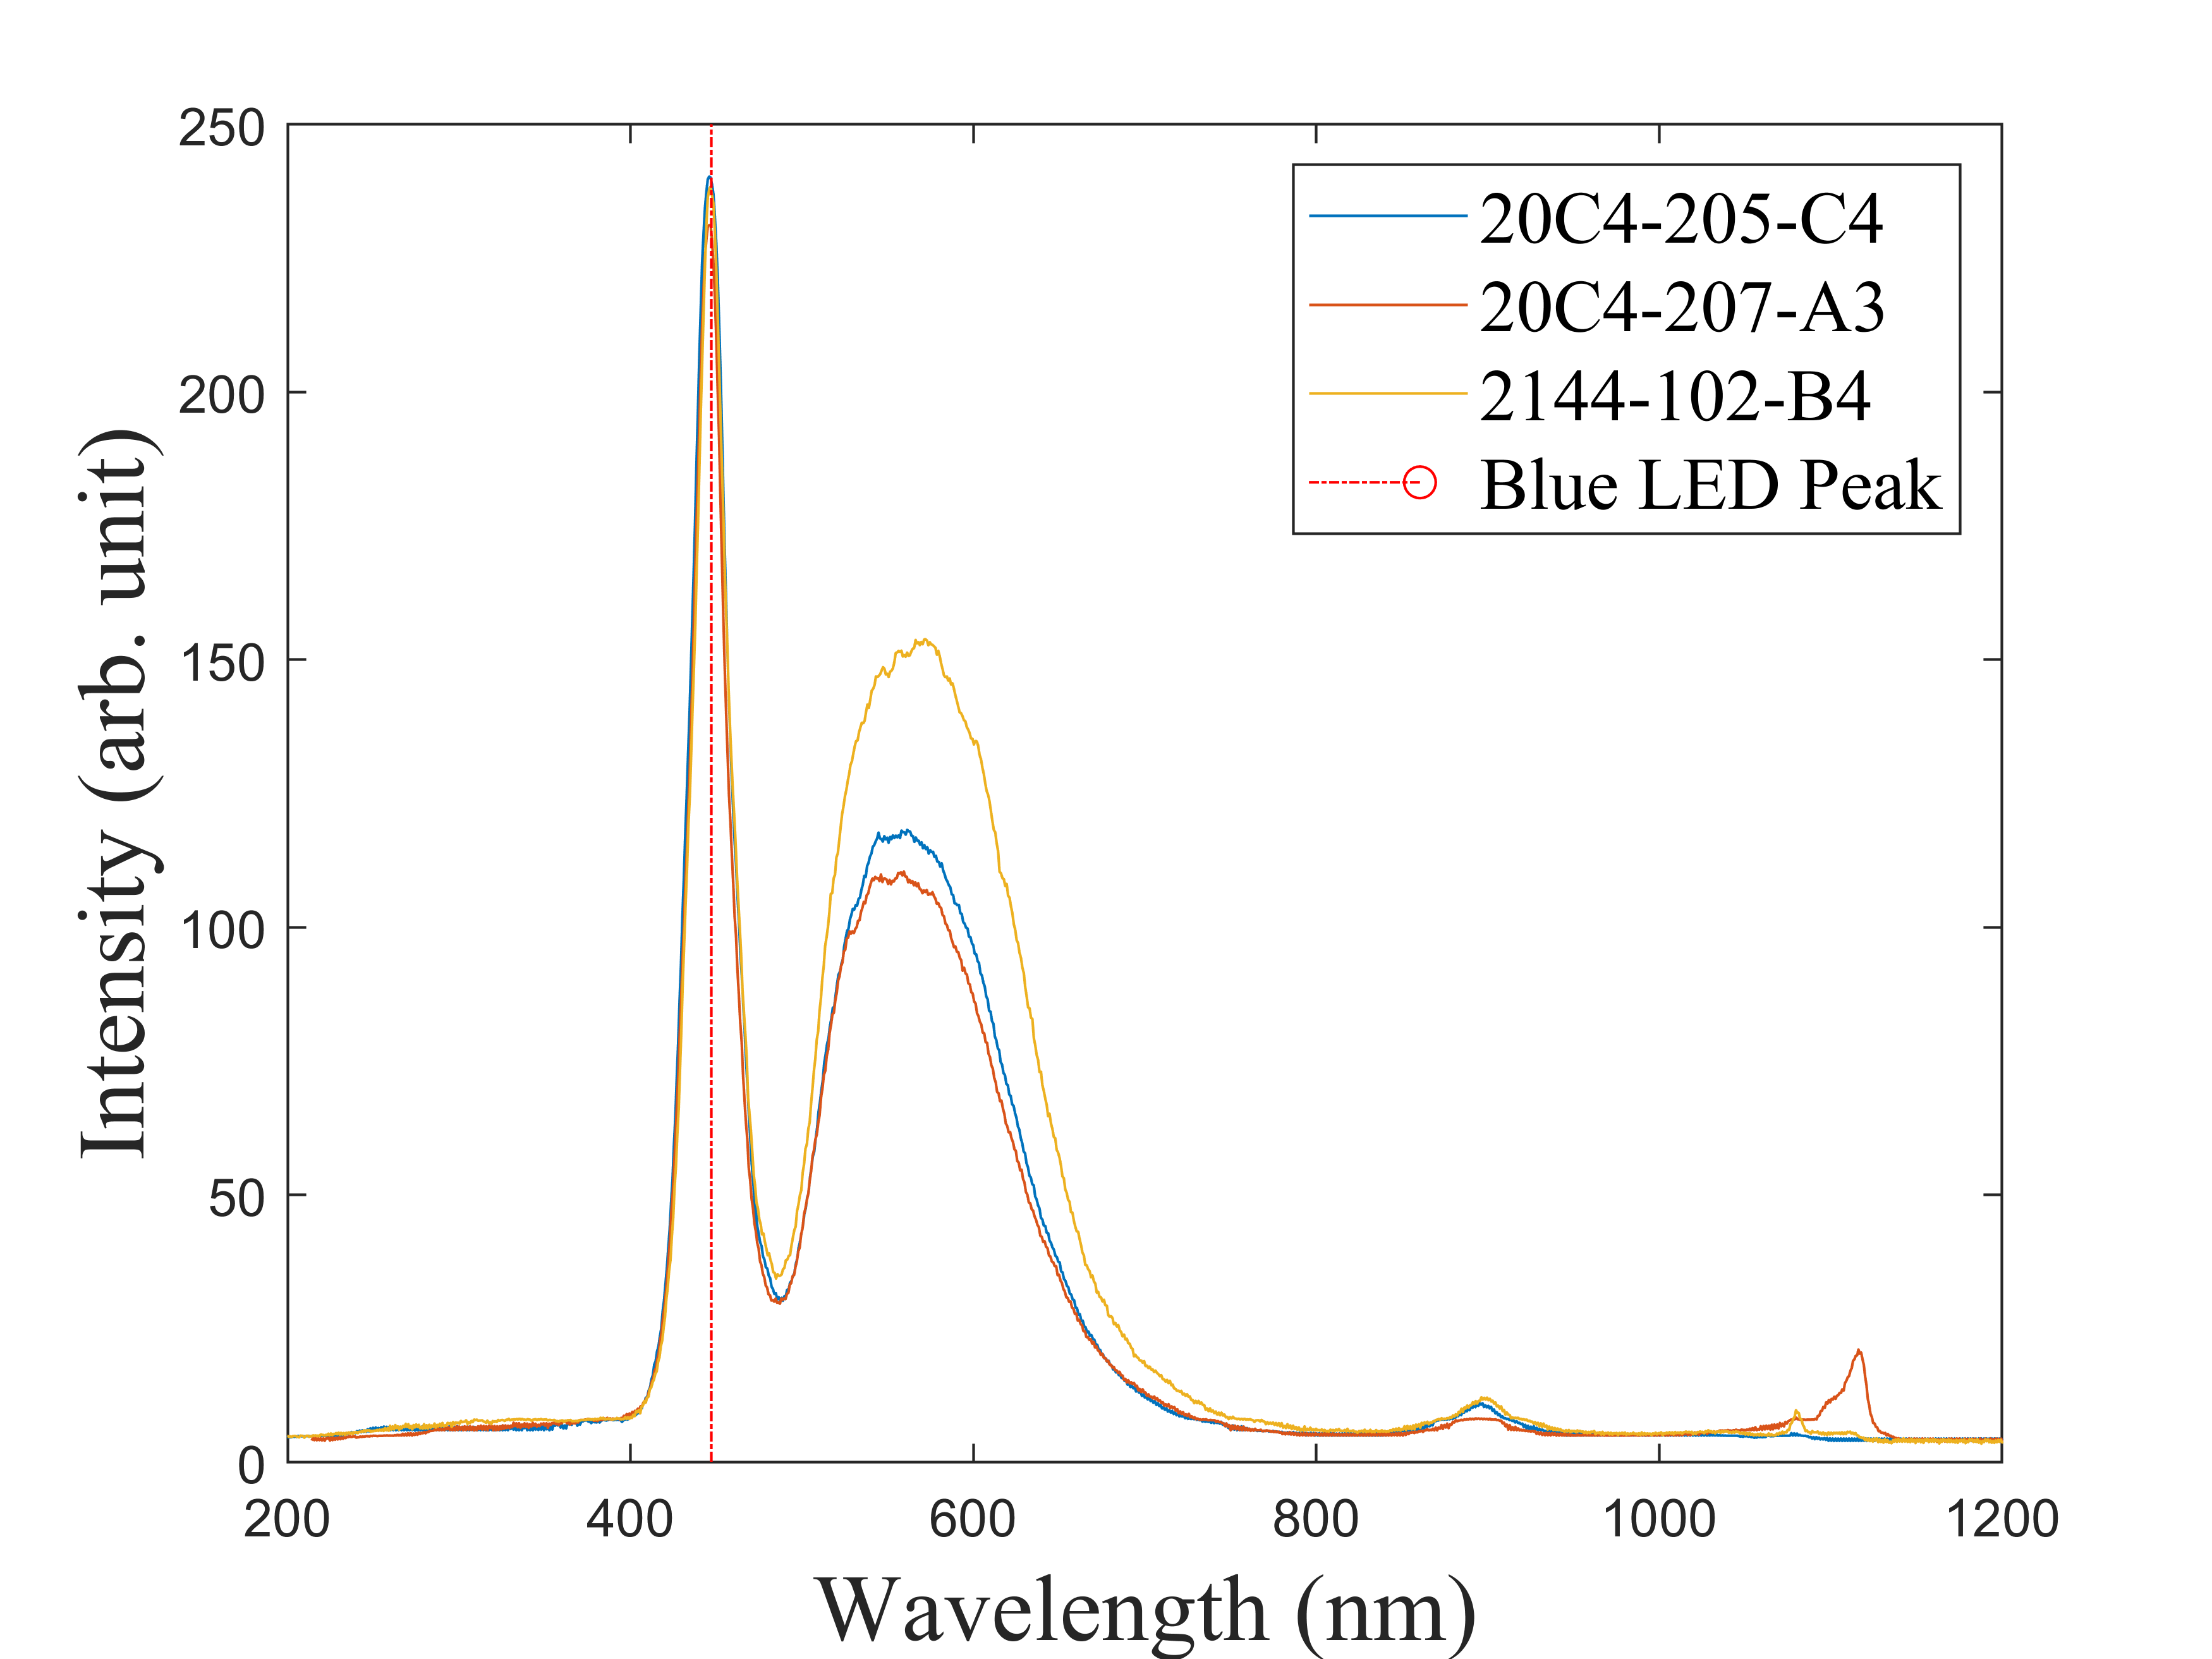
\includegraphics[width=15cm]{figures/Result/白光結果疊圖.png} %插入图片,[]中设置图片大小,{}中是图片文件名
	\caption{三個晶片轉換至波長空間後的白光光譜疊圖} %最终文档中希望显示的图片标题
	\label{三個晶片轉換至波長空間後的白光光譜疊圖} %用于文内引用的标签
\end{figure}
由圖\ref{三個晶片轉換至波長空間後的白光光譜疊圖}. 可知,不同晶片之白光LED光譜,雖因晶片性能與效率不同,而有波形及強度的差異,但經由空間轉換方程式轉換至波長空間後,波長座標位置雖有微小誤差但仍相當精確,因此得證此自動波長校正演算法快速且不失準確度。